% !TEX root = userguide_en.tex
%----------------------------------------------------------
An example of input file for the standard mode is shown below:

\begin{minipage}{10cm}
\begin{screen}
\begin{verbatim}
W = 2
 L = 4
 model = "spin"
 method = "Lanczos"

 lattice = "triangular lattice"
//mu = 1.0
// t = -1.0
// t' = -0.5
// U = 8.0
//V = 4.0
//V'=2.0
J = -1.0
J'=-0.5
// nelec = 8
2Sz = 0
\end{verbatim}
\end{screen}
\end{minipage}
~\\
~\\
~\\
{\bf Basic rules for input files}
\begin{itemize}
\item In each line, there is a set of a keyword (before an ``\verb|=|") and a parameter(after an ``\verb|=|"); 
  they are separated by ``\verb|=|".
\item You can describe keywords in a random order.
\item Empty lines and lines beginning in a ``\verb|//|''(comment outs) are skipped.
\item Upper- and lowercase are not distinguished.
  Double quotes and blanks are ignored.
\item There are three kinds of parameters.\\ 
  1.~Parameters that must be specified~(if not, $\HPhi$ will stop with error messages),\\ 
  2.~Parameters that is not necessary be specified~(if not, default values are used),\\
  3.~Parameters that must not be specified~(if specified, $\HPhi$ will stop with error messages).\\
  An example of 3 is transfer $t$ for the Heisenberg spin system. 
  If you choose ``model=spin", you should not specify ``$t$".
\end{itemize}

We explain each keywords as follows:

\subsection{Parameters about the kind of a calculation}

\begin{itemize}

\item \verb|model|

{\bf Type :} String (Choose from \verb|"Fermion Hubbard"|, \verb|"Spin"|, \verb|"Kondo Lattice"|, 
\verb|"Fermion HubbardGC"|, \verb|"SpinGC"|, \verb|"Kondo LatticeGC"|)\footnote{GC=Grand Canonical}

{\bf Description :} The target model is specified with this parameter;
above words denote the canonical ensemble of the Fermion in the Hubbard model
\begin{align}
H = -\mu \sum_{i \sigma} c^\dagger_{i \sigma} c_{i \sigma} 
- \sum_{i \neq j \sigma} t_{i j} c^\dagger_{i \sigma} c_{j \sigma} 
+ \sum_{i} U n_{i \uparrow} n_{i \downarrow}
+ \sum_{i \neq j} V_{i j} n_{i} n_{j},
\label{fml4_1_hubbard}
\end{align}
canonical ensemble in the Kitaev-Heisenberg model
\begin{align}
H &= -h \sum_{i} S_{i z} + \Gamma \sum_{i} S_{i x} + D \sum_{i} S_{i z} S_{i z}
\nonumber \\
&+ \sum_{i j} \left( J_{i j x} S_{i x} S_{j x} + J_{i j y} S_{i y} S_{j y} + J_{i j z} S_{i z} S_{j z} 
\right),
\label{fml4_1_spin}
\end{align}
canonical ensemble in the Kondo lattice model
\begin{align}
H = - \mu \sum_{i \sigma} c^\dagger_{i \sigma} c_{i \sigma} 
- t \sum_{\langle i j \rangle \sigma} c^\dagger_{i \sigma} c_{j \sigma} 
+ \frac{J}{2} \sum_{i} \left\{
S_{i}^{+} c_{i \downarrow}^\dagger c_{i \uparrow}
+ S_{i}^{-} c_{i \uparrow}^\dagger c_{i \downarrow}
+ S_{i z} (n_{i \uparrow} - n_{i \downarrow})
\right\},
\label{fml4_1_kondo}
\end{align}
grand canonical ensemble of the Fermion in the Hubbard model [Eqn. (\ref{fml4_1_hubbard})],
grand canonical ensemble in the Kitaev-Heisenberg model [Eqn. (\ref{fml4_1_spin})],
and
grand canonical ensemble in Kondo lattice model [Eqn. (\ref{fml4_1_kondo})]
respectively.

\item \verb|method|
  
{\bf Type :} String (Choose from \verb|"Lanczos|", \verb|"TPQ"|, \verb|"Full Diag"|)

{\bf Description :} The calculation type is specified with this parameter;
above words denote 
the single eigenstate calculation by using the Lanczos method,
at the finite-temperature by thermally pure quantum state,
and the full diagonalization method,
respectively.

\item \verb|lattice|

{\bf Type :} String (Choose from \verb|"Chain Lattice"|, \verb|"Square Lattice"|, 
\verb|"Triangular Lattice"|, \verb|Honeycomb Lattice|)

{\bf Description :} The lattice shape is specified with this parameter;
above words denote
the one dimensional chain lattice (Fig. \ref{fig_chap04_1_lattice}(a)), 
the two dimensional square lattice (Fig. \ref{fig_chap04_1_lattice}(b)),
the two dimensional triangular lattice (Fig. \ref{fig_chap04_1_lattice}(c)),
and
the two dimensional anisotropic honeycomb lattice (Fig. \ref{fig_chap04_1_honeycomb}),
respectively.

\begin{figure}[!htbp]
  \begin{center}
    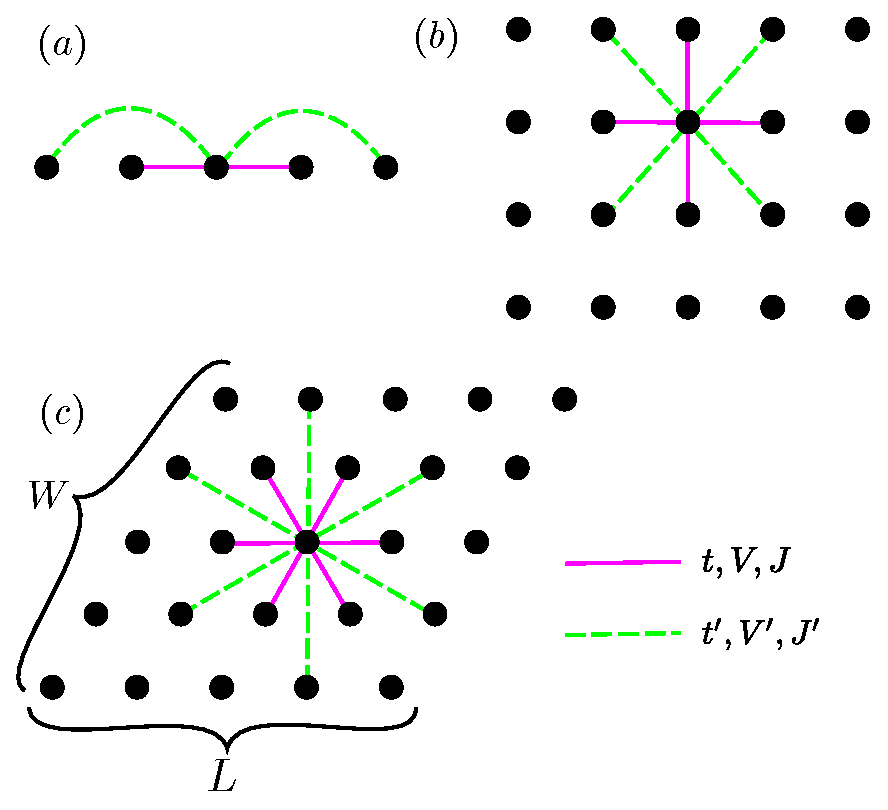
\includegraphics[width=8cm]{../figs/chap04_1_lattice.eps}
    \caption{Schematic illustration of
      (a) one dimensional chain lattice, 
      (b) two dimensional square lattice, and 
      (c) two dimensional triangular lattice.
      They have $t$, $V$, and $J$ as a nearest neighbor hopping, an offsite Coulomb integral, 
      and a spin-coupling constant, respectively (magenta solid lines);
      They also have $t'$, $V'$, and $J'$ as a next nearest neighbor hopping, offsite Coulomb integral, 
      and spin-coupling constant, respectively (green dashed line).
    }
    \label{fig_chap04_1_lattice}
  \end{center}
\end{figure}

\begin{figure}[!htbp]
  \begin{center}
    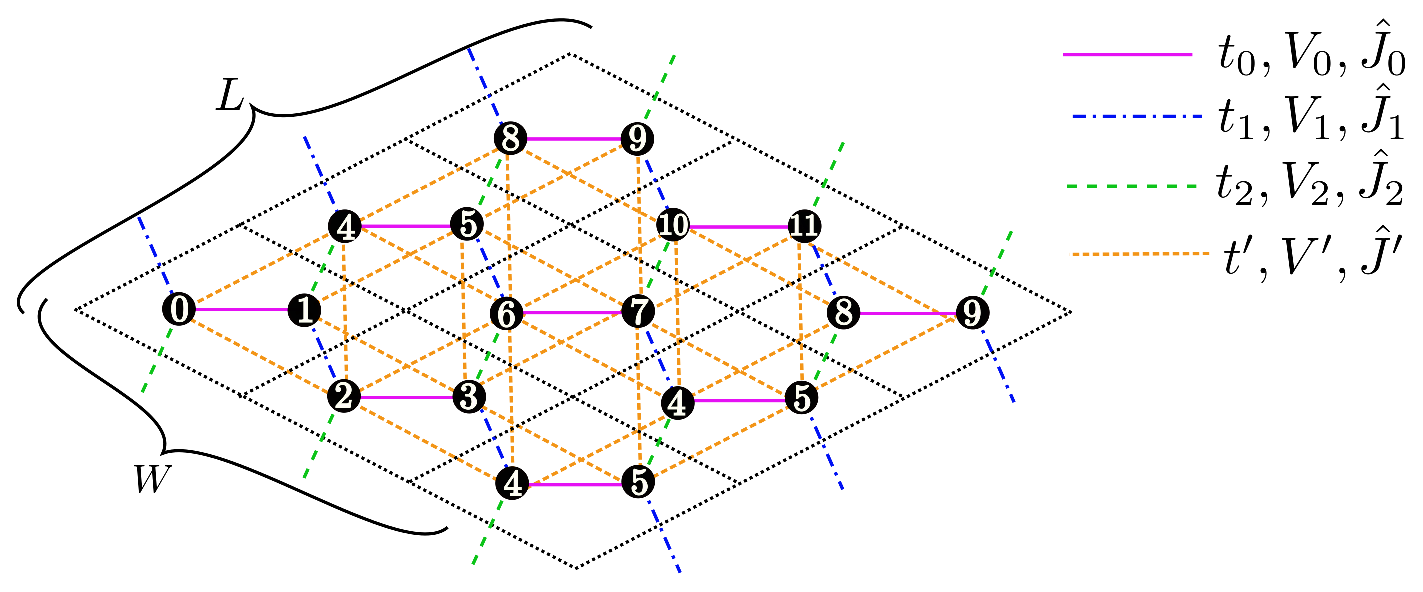
\includegraphics[width=15cm]{../figs/chap04_1_honeycomb.eps}
    \caption{Schematic illustration of the anisotropic honeycomb lattice.
      The nearest neighbor 
      hopping integral, spin coupling, offsite Coulomb integral
      depend on the bond direction.
      Those between second nearest neighbor sites are not supported.
    }
    \label{fig_chap04_1_honeycomb}
  \end{center}
\end{figure}

\end{itemize}

\subsection{Parameters for the lattice}

\begin{itemize}
\item \verb|L|

{\bf Type :} Positive integer

{\bf Description :} The number of
sites along the first dimensional direction
is specified with this parameter.

\item \verb|W|

{\bf Type :} Positive integer

{\bf Description :} The number of
sites along the second dimensional direction
is specified with this parameter.
When \verb|lattice = "Chain Lattice"|, 
it should not be specified because it will not be used
(if specified, $\HPhi$ will stop).

\item \verb|a|

{\bf Type :} Real (\verb|1.0| as a default)

{\bf Description :} The lattice constant is specified with this parameter.
\end{itemize}

\subsection{Parameters for conserved quantities}

\begin{itemize}
\item \verb|nelec|

{\bf Type :} Positive integer

{\bf Description :} The number of valence electrons is specified with this parameter.
When \verb|lmodel = "Fermion HubbardGC"|, \verb|"Spin"|, or  \verb|"SpinGC"|, 
it should not be specified.

\item \verb|2Sz|

{\bf Type :} Integer

{\bf Description :} The $z$ component of the twofold total spin is 
specified with this parameter.
When \verb|lmodel = "Fermion HubbardGC"| or \verb|SpinGC|,
it should not be specified.
\end{itemize}

\subsection{Parameters for the Hubbard model}
\begin{itemize}
\item \verb|mu|

{\bf Type :} Real (\verb|0.0| as a default)

{\bf Description :} The chemical potential $\mu$ (including the site potential)
is specified with this parameter.

\item \verb|t|

{\bf Type :} Real (\verb|1.0| as a default)

{\bf Description :} The nearest neighbor hopping $t$ (See Fig. \ref{fig_chap04_1_lattice})
is specified with this parameter.

\item \verb|t'|

{\bf Type :} Real (\verb|0.0| as a default)

{\bf Description :} The second nearest neighbor hopping $t'$ (See Fig. \ref{fig_chap04_1_lattice})
is specified with this parameter.

\item \verb|t0|, \verb|t1|, \verb|t2|

{\bf Type :} Real (\verb|t| as defaults)

{\bf Description :} The nearest neighbor hopping 
in the anisotropic honeycomb lattice 
(See Fig. \ref{fig_chap04_1_honeycomb})
is specified with this parameter.

\item \verb|U|

{\bf Type :} Real (\verb|0.0| as a default)

{\bf Description :} The onsite Coulomb integral $U$ is specified with this parameter.

\item \verb|V|, \verb|V'|

{\bf Type :} Real (\verb|0.0| as defaults)

{\bf Description :} The nearest neighbor offsite Coulomb integrals $V$
and the second nearest neighbor offsite Coulomb integrals $V'$
(Fig. \ref{fig_chap04_1_lattice} are specified with these parameters.

\item \verb|V0|, \verb|V1|, \verb|V2|

{\bf Type :} Real (\verb|V| as defaults)

{\bf Description :} Nearest neighbor offsite Coulomb integrals 
on the anisotropic honeycomb lattice
(Fig. \ref{fig_chap04_1_honeycomb} are specified with these parameters.

\end{itemize}

\subsection{Parameters for the Kitaev-Heisenberg model}
\begin{itemize}
\item \verb|h|, \verb|Gamma|, \verb|D|

{\bf Type :} Real (\verb|0.0| as a default)

{\bf Description :} The longitudinal magnetic field, transverse magnetic field, 
and the single-site anisotropy parameter are specified with these parameters.

\item \verb|J|

{\bf Type :} Real (\verb|1.0| as a default)

{\bf Description :} The isotropic spin-coupling constant between nearest neighbor sites
(See Fig. \ref{fig_chap04_1_lattice}) is specified with this parameter.
\verb|Jx|, \verb|Jy|, \verb|Jz|, and \verb|Jxy| and set to \verb|J|
if \verb|J| is specified AND none of \verb|Jx|, \verb|Jy|, \verb|Jz| and \verb|Jxy| is specified.

\item \verb|Jz|, \verb|Jxy|

{\bf Type :} Real (\verb|J| as a default)

{\bf Description :} The uniaxially anisotropic spin-coupling constant between nearest neighbor sites
(See Fig. \ref{fig_chap04_1_lattice}) is specified with this parameter.
\verb|Jx| and \verb|Jy| are set to \verb|Jxy|
if \verb|Jxy| is specified AND none of \verb|Jx| and \verb|Jy| is specified.

\item \verb|Jx|, \verb|Jy|

{\bf Type :} Real (\verb|Jxy| as a default)

{\bf Description :} The fully anisotropic spin-coupling constant between nearest neighbor sites
(See Fig. \ref{fig_chap04_1_lattice}) is specified with this parameter.

\item \verb|J'|, \verb|Jx'|, \verb|Jy'|, \verb|Jz'|, \verb|Jxy'|

{\bf Type :} Real (\verb|J'|, \verb|Jxy'|, \verb|Jz'|, \verb|Jx'|, and \verb|Jy'|
are set to  \verb|0.0|,  \verb|J'|, \verb|J'|, \verb|Jxy'|, and \verb|Jxy'| as defaults.)

{\bf Description :} Spin-coupling constants between second nearest neighbor sites
(See Fig. \ref{fig_chap04_1_lattice}) are specified with these parameter.
They are set as 
\verb|J|, \verb|Jx|, \verb|Jy|, \verb|Jz|, and \verb|Jxy| are set.

\item \verb|J0|, \verb|J1|, \verb|J2|, \verb|Jx0|, \verb|Jy0|, \verb|Jz0|, 
  \verb|Jx1|, \verb|Jy1|, \verb|Jz1|, 
  \verb|Jx2|, \verb|Jy2|, \verb|Jz2|, \verb|Jxy0|, \verb|Jxy1|, \verb|Jxy2|

{\bf Type :} Real (
\verb|J| as defaluts for \verb|J0|, \verb|J1|, \verb|J2|. 
\verb|Jxy| as defaults for \verb|Jxy0|, \verb|Jxy1|,  \verb|Jxy2|;
\verb|Jx| as defaults for \verb|Jx0|, \verb|Jx1|, \verb|Jx2|;
\verb|Jy| as defaults for \verb|Jy0|, \verb|Jy1|, \verb|Jy2|;
\verb|Jz| as defaults for \verb|Jz0|, \verb|Jz1|, \verb|Jz2|.)

{\bf Description :} Spin-coupling constants between nearest neighbor sites
in the anisotropic honeycomb lattice
(See Fig. \ref{fig_chap04_1_honeycomb}) are specified with these parameter.

\end{itemize}

\subsection{Parameters for the Kondo model}
\begin{itemize}
\item \verb|mu|

{\bf Type :} Real (\verb|0.0| as a default)

{\bf Description :} The chemical potential $\mu$ (including the site potential)
is specified with this parameter.

\item \verb|t|

{\bf Type :} Real (\verb|1.0| as a default)

{\bf Description :} The nearest neighbor hopping $t$ (See Fig. \ref{fig_chap04_1_lattice})
is specified with this parameter.

\item \verb|t0|, \verb|t1|, \verb|t2|

{\bf Type :} Real (\verb|t| as defaults)

{\bf Description :} The nearest neighbor hopping 
in the anisotropic honeycomb lattice 
(See Fig. \ref{fig_chap04_1_honeycomb})
is specified with this parameter.

\item \verb|J|

{\bf Type :} Real(\verb|0.0| as a default)

{\bf Description :} The spin-coupling constant between the valence and the local electrons
is specified with this parameter.

\end{itemize}

\subsection{Parameters for the numerical condition}
\begin{itemize}
\item \verb|Lanczos_max|

{\bf Type :} Positive integer (\verb|2000| as a default)

{\bf Description :} Upper limit of the Lanczos step is specified with this parameter.

\item \verb|initial_iv|

{\bf Type :} Positive integer (\verb|1| as a default)

{\bf Description :} The non-zero components of an initial vector is specified with this parameter. 
For grand canonical ensemble, the random vector is used as initial vector. 

\item \verb|nvec|

{\bf Type :} Positive integer (\verb|1| as a default)

{\bf Description :} We specify the number of getting 
eigenvalues from the ground energy by Lanczos method.\\
When nvec=2, we obtain the ground-state energy and energy of the first-excited state.

\item \verb|exct|

{\bf Type :} Positive integer (\verb|1| as a default)

{\bf Description :}  We specify the number of getting eigenvectors from the ground energy by Lanczos method.\\
When exct=2, we obtain the eigenvector of the first-excited state.

{\bf Note}:  the following condition must be satisfied: \verb|nvec| $>=$ \verb|exct|.

\item \verb|LanczosEps|

{\bf Type :} Positive Integer (\verb|14| as a default)

{\bf Description :} The convergence criteria for the Lanczos method is specified with this parameter.
If the difference between the old and the new target eigenvalue fall below $10^{- \verb|LanczosEps|}$, 
the Lanczos step will finish.

\item \verb|LancczosTarget|

{\bf Type :} Positive integer (\verb|2| as a default)

{\bf Description :} We specify the target eigenenergy for the convergence criteria.
If this set to \verb|1|, target eigenenergy becomes the ground state.

\item \verb|LargeValue|

{\bf Type :} Integer (The default value is written below.)

{\bf Description :} (Only for TPQ) 
We use $l$ as $l-\hat{H}/N_{s}$ in the TPQ calculation.
Usually, the largest eigenvalue of Hamiltonian is used as $l$. 
Thus, we take the default value of $l$ for each models is as follows:

\begin{itemize}

\item Hubbard model [Eqn. (\ref{fml4_1_hubbard})]

The canonical ensemble
\begin{align}
l = |\mu| \frac{N_{\rm elec}}{N_{\rm site}}
+ 2 z |t| + 2 z' |t'| + |U| + 2 z |V| + 2 z' |V'| 
\end{align}
The grand canonical ensemble
\begin{align}
l = 2|\mu|
+ 2 z |t| + 2 z' |t'| + |U| + 2 z |V| + 2 z' |V'|
\end{align}

\item Kitaev-Heisenberg model [Eqn. (\ref{fml4_1_spin})]

The canonical ensemble
\begin{align}
l = \frac{1}{2}|h| + \frac{1}{2}|D| + \frac{1}{4}|\Gamma|
+\frac{z}{8} (|J_x|+|J_y|+|J_z|) +\frac{z'}{8} (|J'_x|+|J'_y|+|J'_z|) 
\end{align}
The grand canonical ensemble
\begin{align}
l = \frac{|S_z^{\rm tot}|}{N_{\rm site}}|h| + \frac{1}{2}|D| + \frac{1}{4}|\Gamma|
+\frac{z}{8} (|J_x|+|J_y|+|J_z|) +\frac{z'}{8} (|J'_x|+|J'_y|+|J'_z|)
\end{align}

\item Kondo lattice model [Eqn. (\ref{fml4_1_kondo})]

The canonical ensemble
\begin{align}
l = |\mu| \frac{N_{\rm elec}}{N_{\rm site}} + 2 z |t| + \frac{1}{4} |J| 
\end{align}
The grand canonical ensemble
\begin{align}
l = 2|\mu| + 2 z |t| + \frac{1}{4} |J| 
\end{align}

\end{itemize}

\item \verb|NumAve|

{\bf Type :} Positive integer (\verb|5| as a default)

{\bf Description :} (Only for the TPQ) The number of independent runs for the TPQ method is specified 
with this parameter.

\item \verb|ExpecInterval|

{\bf Type :} Positive integer (\verb|20| as a default)

{\bf Description :} (Only for the TPQ) 
We specify the interval steps of calculating correlation functions in TPQ method.\\ 
{\bf Note:} The small interval increases the time cost of calculations.

\end{itemize}


